\chapter{Implementation Details}
\label{ch:impl}

This chapter documents the module-wise implementation of the
proposed system and presents annotated snapshots of the running UI.
The full source code is released open-source at
\url{https://github.com/DeepPatange/AI-Stroy-Generator}.

\section{Project Layout}
The repository is structured as follows:

\begin{lstlisting}
AI-Story-Generator/
|-- main.py                    # FastAPI entry point, 14 endpoints
|-- config.py                  # Provider, model, temperature config
|-- requirements.txt           # Python dependencies
|-- app/
|   |-- modules/
|   |   |-- user_input.py            # 17 questions, 4 phases
|   |   |-- context_extraction.py    # StoryContext + custom_elements
|   |   |-- knowledge_memory.py      # SQLite + LRU cache
|   |   |-- prompt_engineering.py    # 6 prompt families
|   |   |-- story_generator.py       # BaseLLMClient + 4 providers
|   |   |-- story_flow_manager.py    # 5-phase FSM + trackers
|   |   `-- output_formatter.py      # TXT/MD/HTML export
|   |-- templates/index.html         # Jinja2 SPA shell
|   `-- static/
|       |-- css/style.css            # CSS custom-property themes
|       `-- js/app.js                # StoryForgeApp class (~1.7 kLOC)
`-- data/                            # SQLite db
\end{lstlisting}

\section{Module-wise System Implementation}

\subsection{Module 1: User Input Acquisition}
The user-input module exposes the question pool to the frontend via
two REST endpoints (\texttt{/api/questions/all} for phase-grouped
batch retrieval and \texttt{/api/question/next} for legacy sequential
mode) and accepts responses via \texttt{POST /api/response}. The
landing page (Figure~\ref{fig:ui-landing}) lets the user pick a
budget; the question form (Figure~\ref{fig:ui-form}) renders every
question with multiple-choice options plus a dashed
\emph{``Write my own''} chip for custom answers.

\begin{figure}[H]
    \centering
    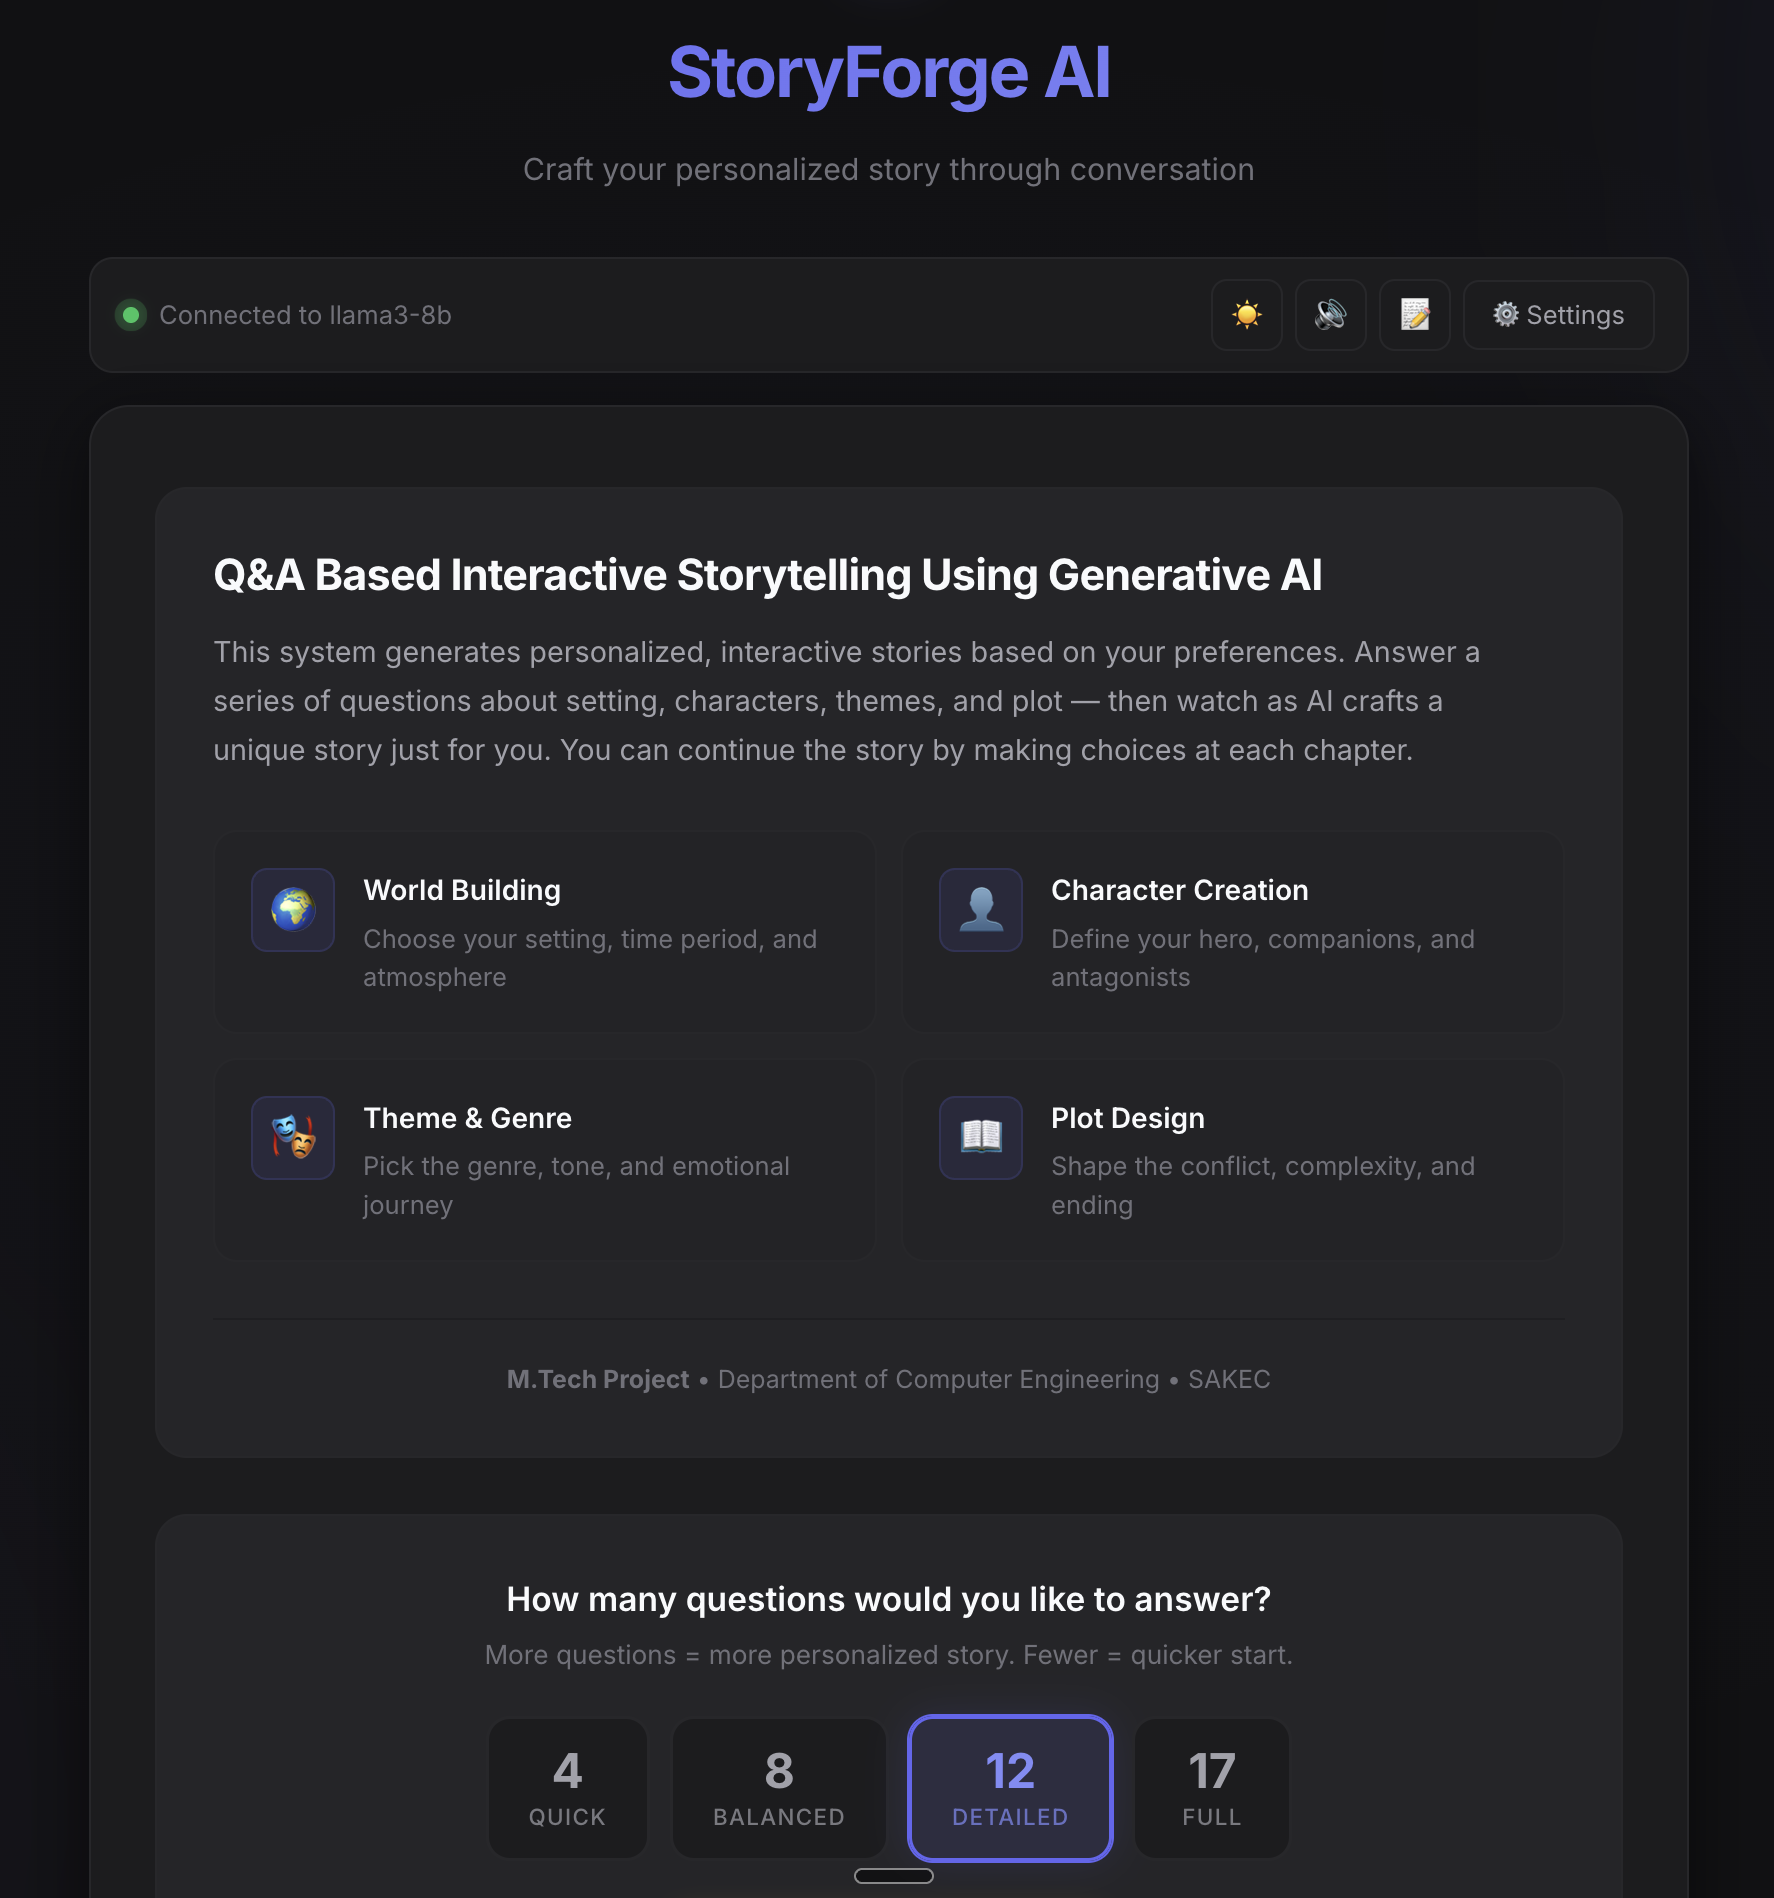
\includegraphics[width=0.85\textwidth]{images/s01_landing.png}
    \caption{Landing page.}
    \label{fig:ui-landing}
\end{figure}

\begin{figure}[H]
    \centering
    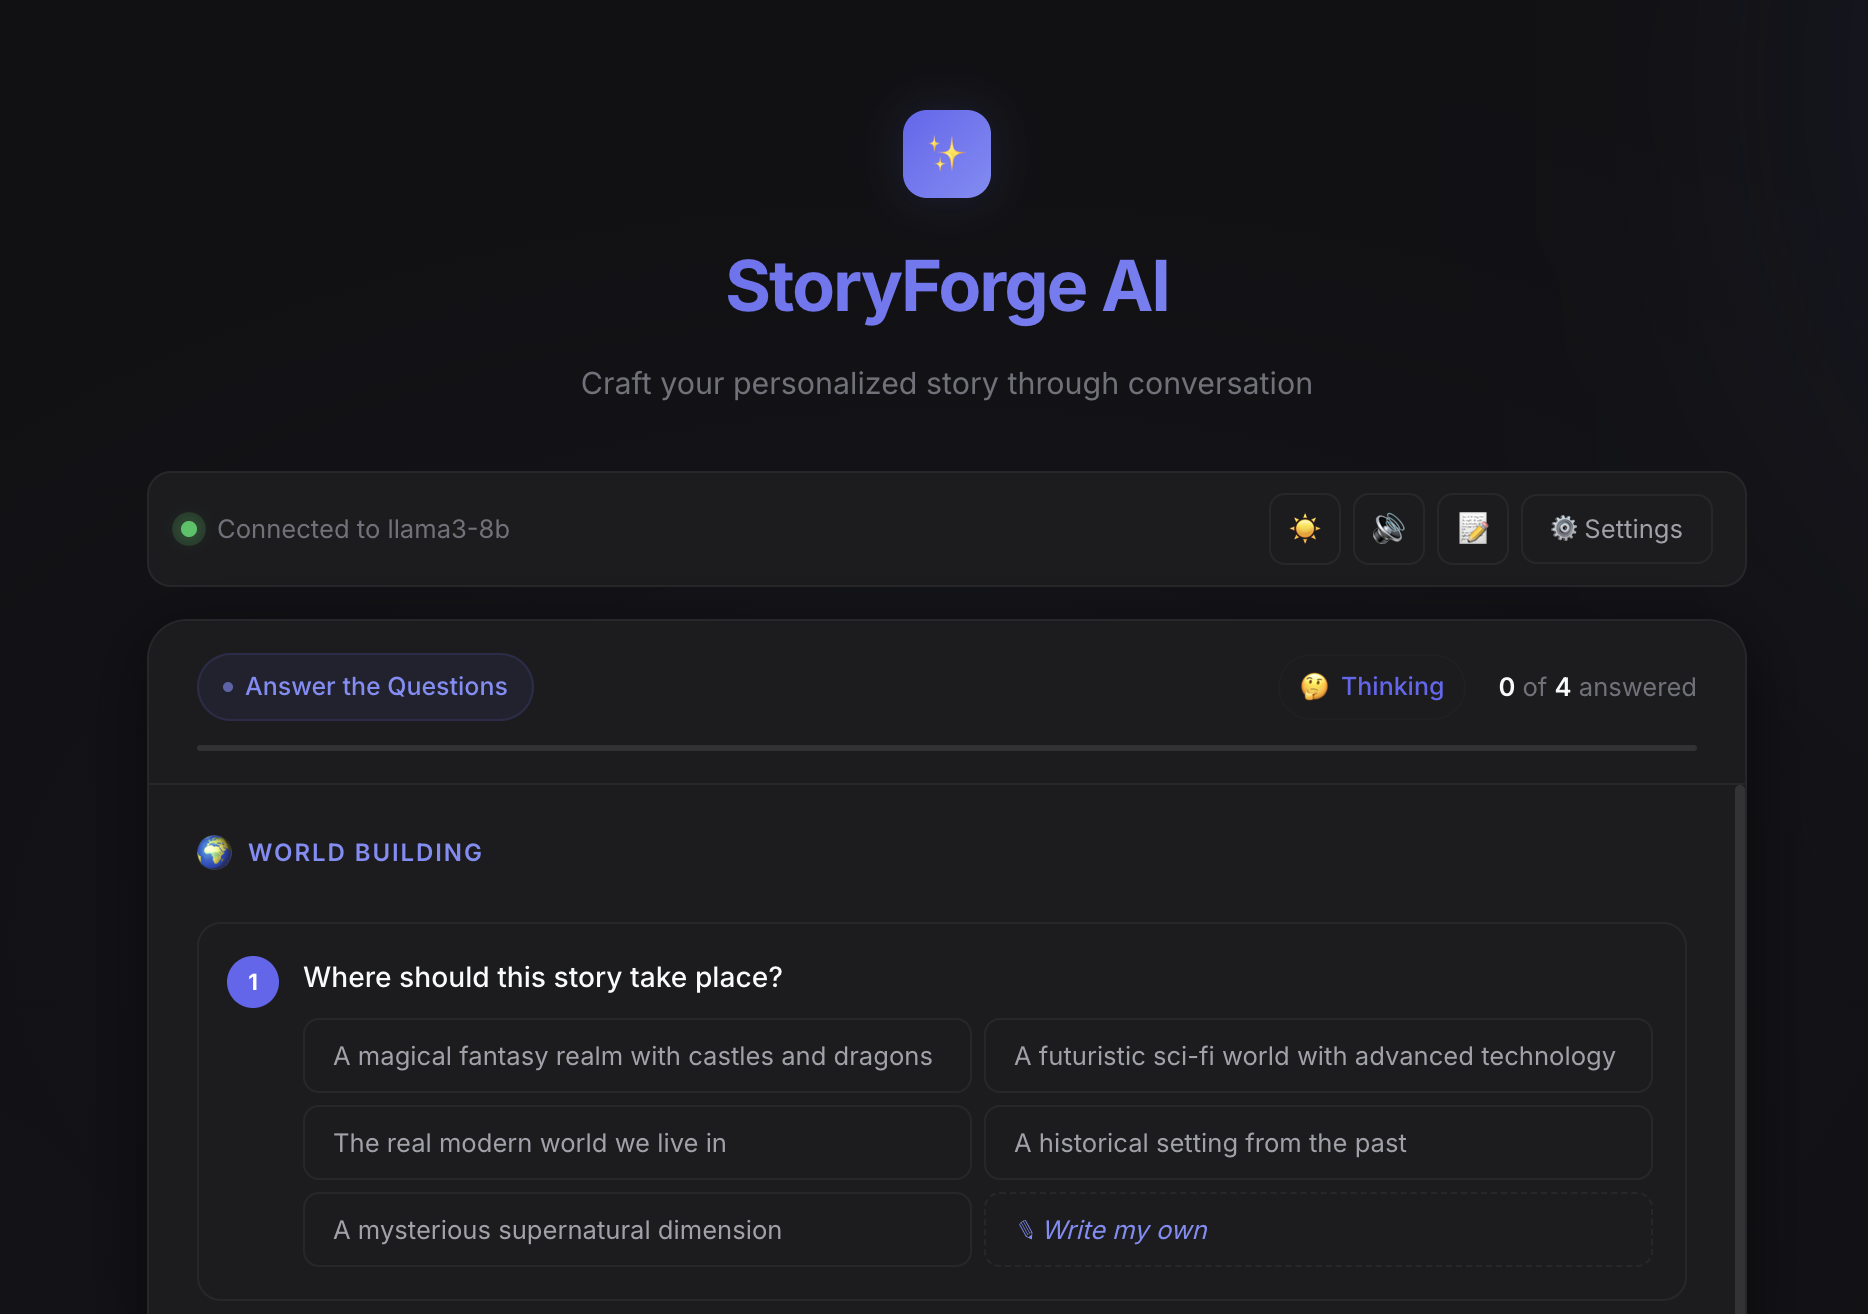
\includegraphics[width=0.85\textwidth]{images/s02_questions.png}
    \caption{Question form.}
    \label{fig:ui-form}
\end{figure}

\subsection{Module 2: Context Extraction Engine}
The context-extraction module projects raw responses into a
\texttt{StoryContext} Pydantic model with explicit fields for
setting, character, theme and plot dimensions. A two-pass pipeline
first classifies answers using keyword dictionaries (6 genres, 5
setting types, 5 conflict types) and then extracts proper-noun
entities via regex. Identifiers prefixed \texttt{custom\_} are
routed into the free-form \texttt{custom\_elements} dictionary;
this is the key plumbing that makes user-added questions flow into
the prompt without code changes:

\begin{lstlisting}[language=Python]
elif question_id.startswith("custom_"):
    self.context.custom_elements[question_id] = answer
\end{lstlisting}

\subsection{Module 3: Knowledge and Memory}
A SQLite3 database stores five tables (\S\ref{ch:proposed}). The
module also maintains an LRU in-memory cache for the active session
and exposes a sliding-window helper:

\begin{lstlisting}[language=Python]
def get_recent_context(session_id: str, k: int = 4) -> str:
    """Return the concatenated text of the last k segments."""
\end{lstlisting}

\subsection{Module 4: Prompt Engineering}
Six prompt templates are interpolated with \texttt{StoryContext}
fields, with genre-specific guidance injected (fantasy: magical
systems; mystery: clue placement and red herrings; romance:
emotional pacing). After the templated prompt $T(\mathbf{c})$ is
built, the module appends user-added preferences:

\begin{lstlisting}[language=Python]
if context.custom_elements:
    extras = "\n".join(f"- {v}" for v in context.custom_elements.values() if v)
    if extras:
        prompt += "\n\nAdditional user preferences to honour:\n" + extras
\end{lstlisting}

\subsection{Module 5: Story Generator (LLM)}
The story generator implements an abstract base class
\texttt{BaseLLMClient} with four concrete subclasses. A factory
selects the active client based on \texttt{LLM\_PROVIDER}. The
Settings panel (Figure~\ref{fig:ui-settings}) exposes the
provider switch to non-developer users; switching providers issues
\texttt{POST /api/settings} which hot-swaps the underlying client
without restart.

\begin{figure}[H]
    \centering
    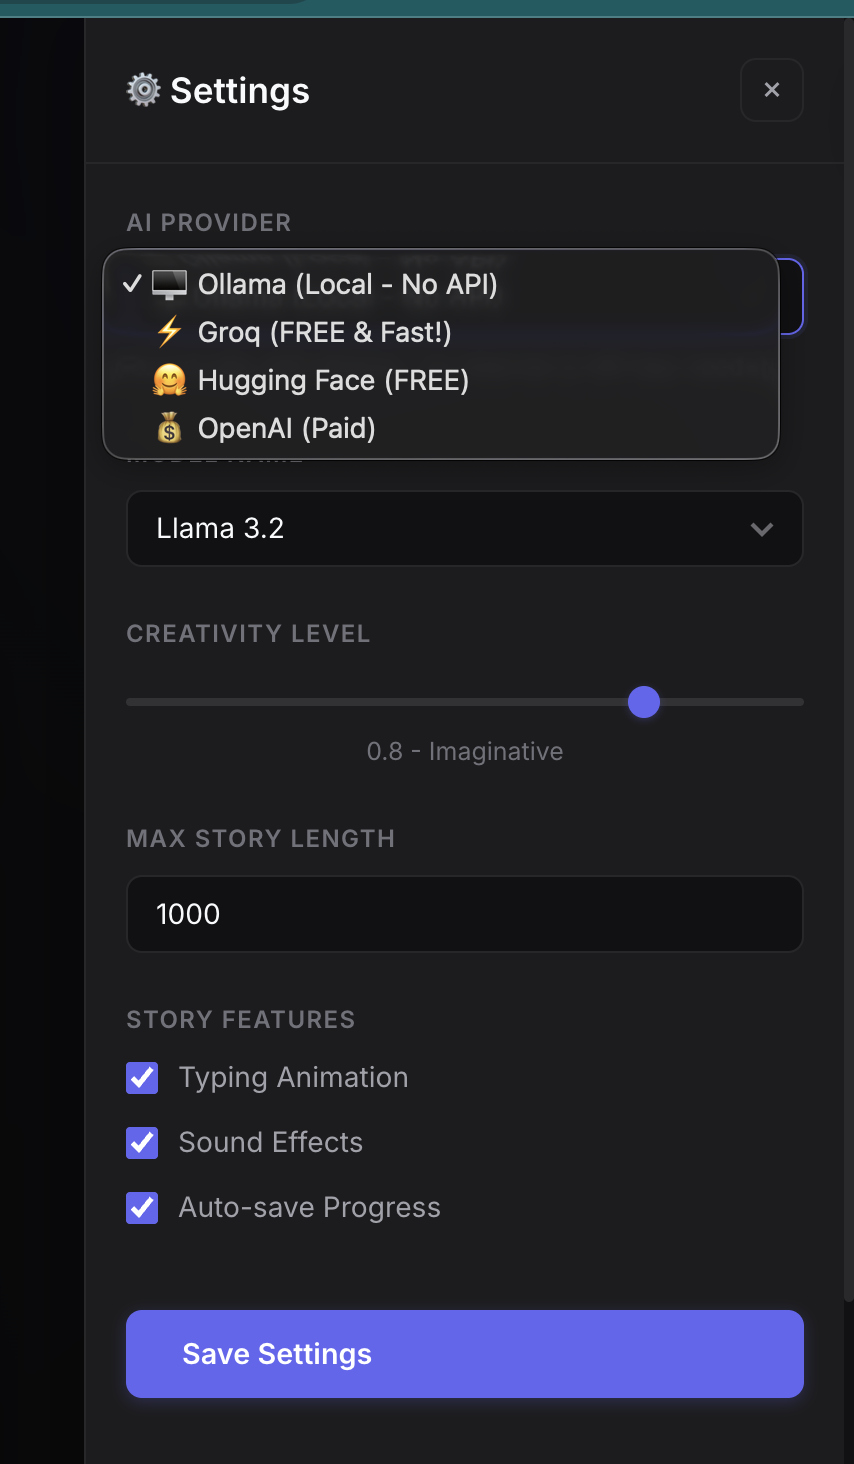
\includegraphics[width=0.55\textwidth]{images/s05_settings.png}
    \caption{Settings panel.}
    \label{fig:ui-settings}
\end{figure}

\subsection{Module 6: Story Flow Manager}
A finite-state machine implementing Freytag's pyramid drives phase
transitions on word-count thresholds (0--400, 400--1200, 1200--1800,
1800--2400, $>$2400). A \texttt{CharacterTracker} monitors mentions
and traits; a \texttt{PlotThreadTracker} flags unresolved threads.

\subsection{Module 7: Output Formatter}
The formatter cleans LLM-emitted text (collapses whitespace, fixes
quote and dash characters), splits content at sentence boundaries,
lifts dialogue to styled HTML spans, and supports three export
formats (TXT, Markdown, HTML).

\section{Multimodal Subsystems}

\subsection{Image Generation (Pollinations.ai)}
The frontend's \texttt{createImageCard()} function builds the prompt
using the sentence-scored extractor described in
\S\ref{ch:proposed}, then dispatches an HTTPS request through the
serial-throttling queue:

\begin{lstlisting}[language=Java]
imageUrlFor(segmentText, seed, opts={}) {
    const prompt = this.buildImagePrompt(segmentText, opts);
    const params = new URLSearchParams({
        width: '768', height: '432', nologo: 'true',
        seed: String(seed)
    });
    return `https://image.pollinations.ai/prompt/${encodeURIComponent(prompt)}?${params}`;
}
\end{lstlisting}

Figure~\ref{fig:ui-loading} shows the loading state during which the
LLM call and image synthesis run concurrently;
Figure~\ref{fig:ui-story} shows the rendered first chapter with the
on-demand scene illustration.

\begin{figure}[H]
    \centering
    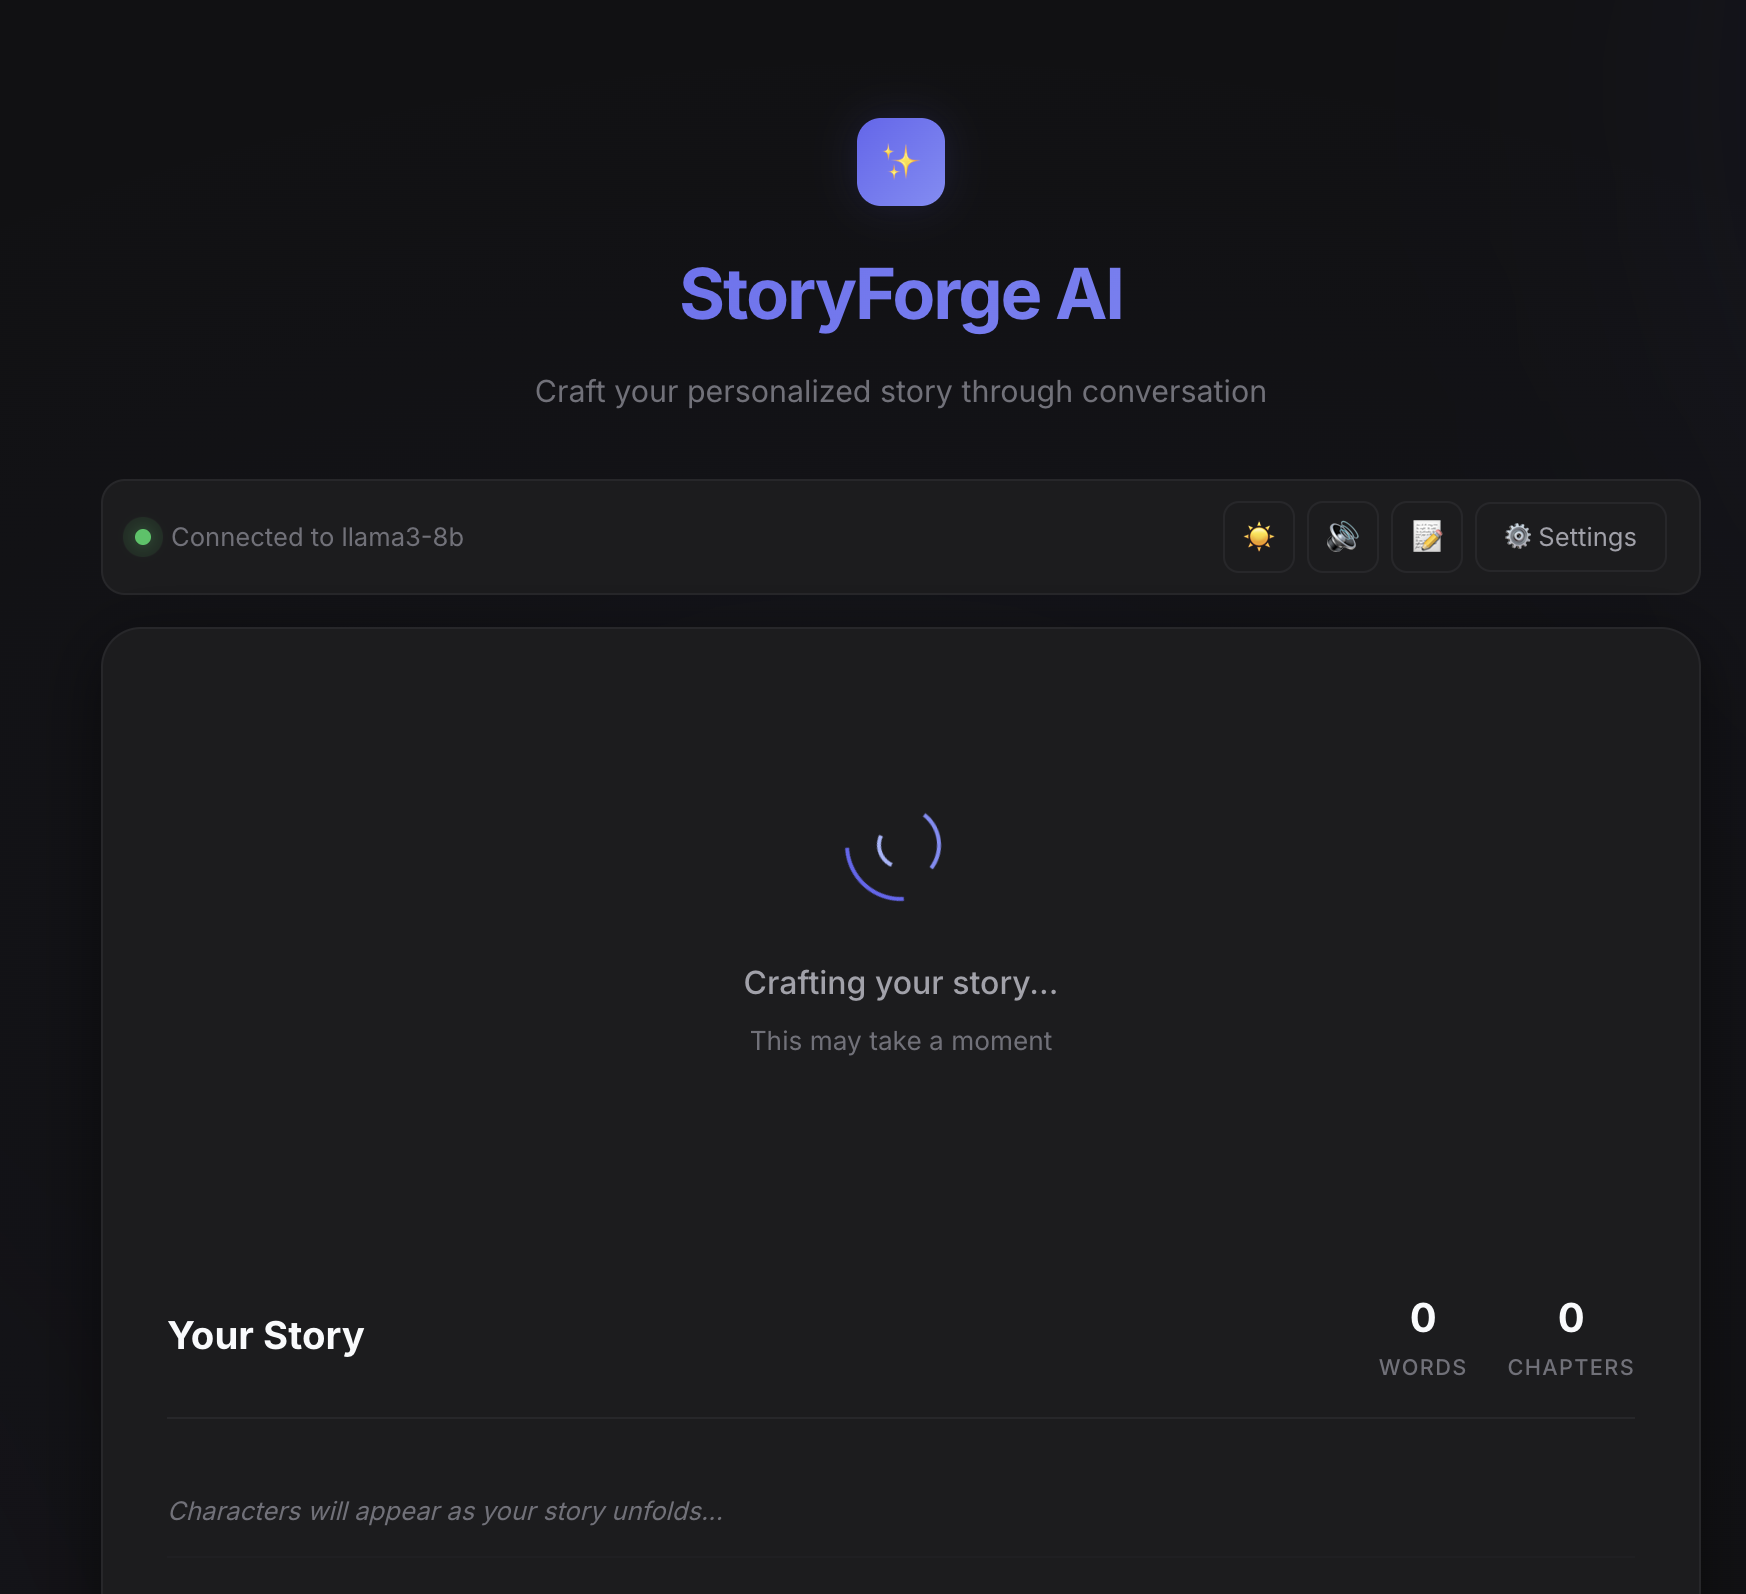
\includegraphics[width=0.85\textwidth]{images/s03_loading.png}
    \caption{Loading state.}
    \label{fig:ui-loading}
\end{figure}

\begin{figure}[H]
    \centering
    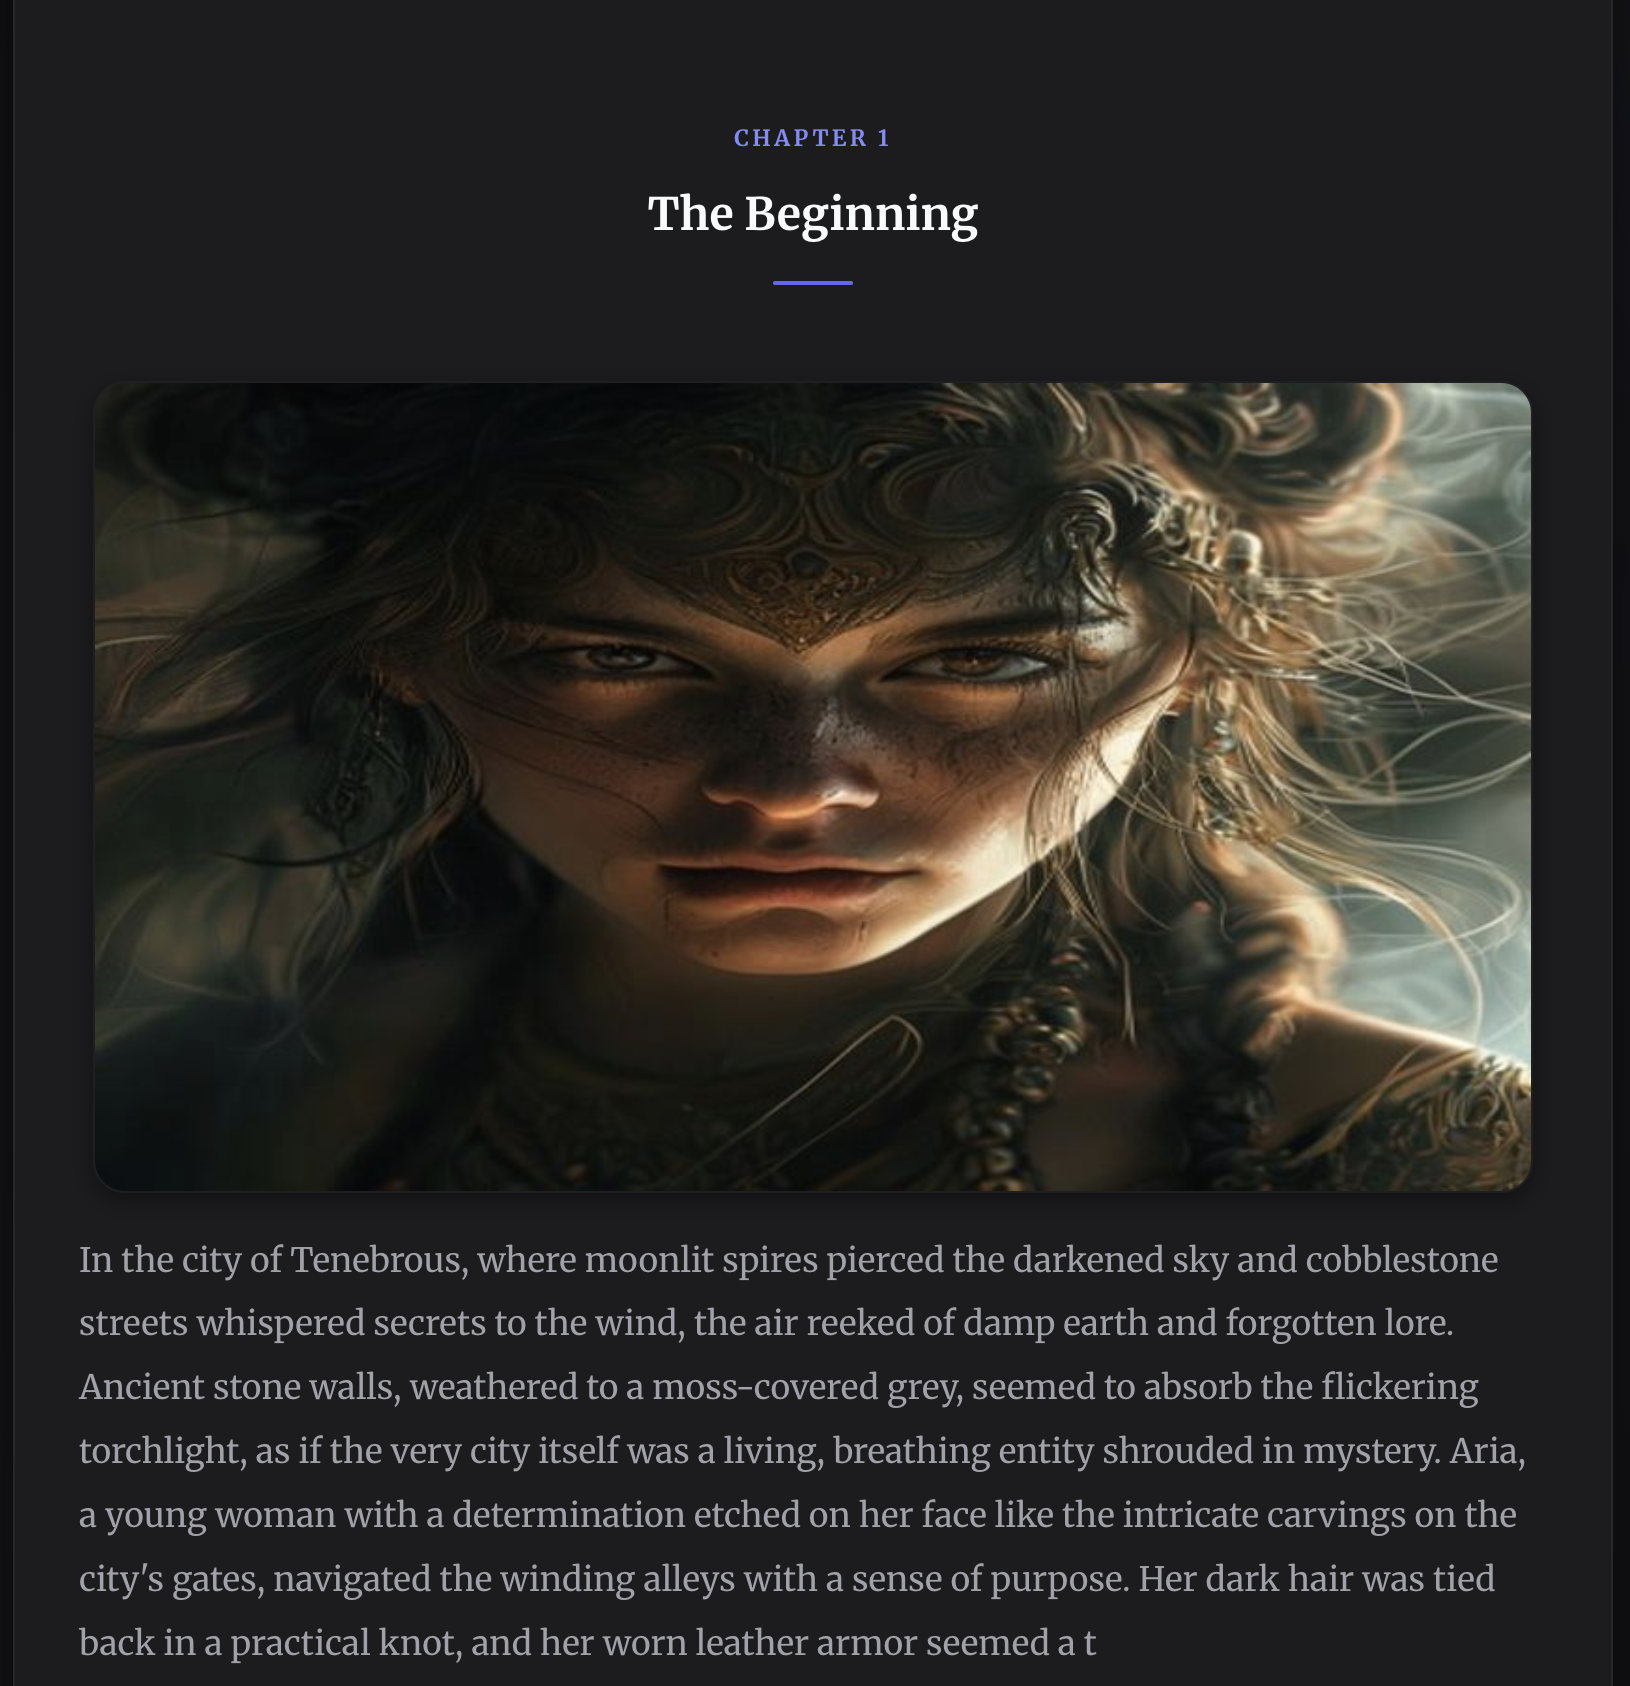
\includegraphics[width=0.65\textwidth]{images/s04_story_image.png}
    \caption{Generated story segment with scene illustration.}
    \label{fig:ui-story}
\end{figure}

\subsection{TTS Narration (Web Speech Synthesis)}
The narration subsystem uses the browser-native
\texttt{window.speechSynthesis} API, queueing one utterance per
segment with pause / resume / stop semantics. No external API key
is required; the voice is whichever the operating system provides
for the active locale.

\subsection{Ambient Music (SoundHelix CDN)}
Eight genre presets map to royalty-free SoundHelix tracks loaded via
\texttt{HTMLAudio} with \texttt{loop=true} and JavaScript volume
ramping for 2.4\,s fade-in and 0.8\,s fade-out. No
\texttt{crossOrigin} attribute is set because the CDN does not return
\texttt{Access-Control-Allow-Origin} headers --- a subtle constraint
discovered during development that broke the first implementation.

\section{Reader Analytics}

\subsection{Story Map (D3 vertical tree)}
The Story Map flattens the chronologically ordered chapters into a
hierarchical tree using \texttt{d3.tree()}. Each node carries an
80-character preview of its chapter and the user choice that led
to it.

\subsection{Character Relationship Graph (D3 force layout)}
The character graph runs a force simulation with link distance 110,
charge $-220$ and a collision radius of 34 pixels. Only characters
with mention count $\geq 2$ are drawn; node radius scales linearly
with mention count. The modal explicitly discloses this is a
co-appearance graph and not a verified relationship-extraction model.

\section{Custom Q\&A Authoring}
Two affordances live in the UI:
\begin{itemize}
    \item Per-question dashed ``Write my own'' chip that toggles a
    textarea; the textarea value overrides any previously-selected
    multiple-choice option.
    \item ``+ Add Your Own Question'' button at the foot of the form
    that opens an inline composer (question + answer); saved entries
    appear as cards with a remove control.
\end{itemize}
Each user-added Q\&A pair is dispatched as a normal response with a
synthetic ID \texttt{custom\_q\_N}; the context-extraction engine
routes such IDs into \texttt{custom\_elements}, and the prompt layer
serialises them as bullets at the end of the prompt.

\section{Code Statistics}
Table~\ref{tab:loc} reports the size of the implementation.

\begin{table}[!t]
\caption{Implementation footprint.}
\label{tab:loc}
\centering
\renewcommand{\arraystretch}{1.1}
\begin{tabular}{@{}lr@{}}
\toprule
\textbf{Component}                                & \textbf{LOC} \\
\midrule
Python backend (7 modules + main + config)        & $\approx$3{,}800 \\
Frontend JavaScript (StoryForgeApp class)         & $\approx$1{,}700 \\
Frontend CSS                                      & $\approx$2{,}200 \\
HTML template                                     & $\approx$400 \\
Tests + tooling                                   & $\approx$300 \\
\midrule
\textbf{Total}                                    & $\approx$\textbf{8{,}400} \\
\bottomrule
\end{tabular}
\end{table}
